\chapter{\scshape Risultati Sperimentali e Analisi Critica}\label{cap:4-risultati}

\section{Dataset e metriche di valutazione}
Un sistema biometrico che decide in pochi secondi se concedere l'accesso a un servizio non può essere giudicato dalla sola impressione d'uso: può nascondere tassi di rifiuto inaccettabili o lasciare passare con regolarità un video riprodotto su un telefono.
Per questo motivo per effettuare la valutazione delle \textbf{performance del sistema}, sono state consegnate al server descritto nel Capitolo~\ref{cap:3-implementazione} un insieme di registrazioni controllate e ripetibili.
Tutte le misure sono state eseguite sullo stesso dispositivo che ospita il backend durante lo sviluppo: un portatile con processore \textbf{Apple M2} (8 core) e \textbf{8 GB} di memoria unificata, sistema operativo macOS 27, alimentazione collegata.
L'ambiente software coincide con quello del server: Python 3.14, InsightFace 2.1, \gls{onnx} Runtime 1.31 e OpenCV 5.0.
Le reti di InsightFace sono eseguite con il provider \textit{CoreMLExecutionProvider}, che delega parte del grafo all'acceleratore neurale del chip. Le latenze sono confrontate anche con l'esecuzione su sola CPU nel Capitolo~\ref{cap:4.3-liveness}.
Le misure sono state raccolte in condizioni d'uso realistiche (con un monitor esterno collegato e altre applicazioni aperte), misurando la memoria come \textit{Resident Set Size} del solo processo di valutazione. 
Quindi la lettura della memoria risente poco di questa scelta, mentre le latenze vanno lette come rappresentative di una macchina di sviluppo \textbf{non dedicata}.

Invece di ripetere a mano decine di accessi dal browser, ogni sessione di \textit{live verification} è stata \textbf{riprodotta offline} a partire da video registrati attraverso uno script di valutazione che simula il comportamento del client descritto nel Capitolo~\ref{cap:3.4-ui}.
Uno script si occupa di aprire il video, estrarre i fotogrammi, comprimerli e inviarli al server con la stessa frequenza di un client reale, mentre un altro script raccoglie le risposte del server e calcola le metriche di performance.
Al termine di ogni verdetto la sessione riparte da capo sullo stesso video, per cui un video di dieci secondi produce circa sette sessioni consecutive da $N = 35$ fotogrammi.
La riproduzione offline comporta due semplificazioni volute:
\begin{itemize}
    \item \textbf{l'assenza del database}: la galleria è costituita dagli embedding di tutte le immagini di documento raccolte, e la ricerca esaustiva sostituisce l'indice \textit{HNSW} di \textit{MongoDB Atlas}, che restituisce lo stesso primo risultato a meno degli errori dell'approssimazione descritti nel Capitolo~\ref{cap:2.4-persistenza}.
    \item \textbf{l'assenza della rete}: il tempo di una sessione è stimato come somma, fotogramma per fotogramma, del massimo tra l'intervallo di campionamento $\Delta$ e il tempo di elaborazione misurato, come formalizzato nell'Equazione~\eqref{eq:tempoSessioneSimulato}
\end{itemize}
In cambio, la stessa registrazione \textbf{può essere rianalizzata} variando un solo parametro alla volta (la lunghezza del buffer, le soglie, il modello o la pre-elaborazione del documento), e ogni esperimento è ripetibile in modo deterministico.

\paragraph{Composizione del dataset}
Il \textbf{dataset reale} è stato progettato privilegiando la profondità delle osservazioni per soggetto rispetto al numero di soggetti: tre volontari, indicati con i codici \textbf{S1}, \textbf{S2} e \textbf{S3}, hanno registrato ciascuno fino a nove condizioni di acquisizione, per un totale di 24 video, 7\,358 fotogrammi analizzati e 190 sessioni simulate.
Essendo S2 e S3 fratelli, la somiglianza tra i due offre un caso naturale di \textbf{impostore difficile}, che verrà ripreso nell'analisi dei confronti.
Tutte le registrazioni sono state acquisite con la stessa fotocamera, la webcam integrata di un MacBook Air M2, tramite il software OBS a $1920 \times 1080$ pixel e 60 fotogrammi al secondo, nella stessa stanza e con le stesse due sorgenti luminose (una luce dall'alto e un faretto laterale) accese o spente a seconda della condizione.
Mantenere costanti dispositivo e ambiente riduce la varietà, ma permette di attribuire le differenze tra le condizioni al solo fattore che di volta in volta viene modificato.
Le condizioni sono state scelte per sollecitare separatamente i fattori indicati come critici nel Capitolo~\ref{cap:1-fondamenti}: sono riassunte nella Tabella~\ref{tab:condizioniAcquisizione}.
\begin{table}[htbp]
    \centering
    \footnotesize
    \renewcommand{\arraystretch}{1.25}
    \begin{tabular*}{\textwidth}{@{\extracolsep{\fill}}llcc@{}}
        \hline
        \textbf{Codice} & \textbf{Condizione} & \textbf{Fotogrammi} & \textbf{Sessioni} \\
        \hline
        V1 & Luce normale, movimento naturale & 807 & 22 \\
        V2 & Soggetto immobile\footnotemark~(atteso \texttt{STATIC\_FACE}) & 654 & 17 \\
        V3 & Rotazione lenta della testa (\textit{yaw} e \textit{pitch}) & 1\,138 & 30 \\
        V4 & Poca luce (solo faretto laterale) & 855 & 23 \\
        V5 & Controluce (faretto alle spalle) & 838 & 20 \\
        V6 & Distanza variabile dalla fotocamera & 1\,095 & 27 \\
        V7 & Senza occhiali & 904 & 25 \\
        V8 & Movimenti ampi del corpo & 888 & 21 \\
        V9 & Espressioni accentuate (lingua, bocca aperta) & 179 & 5 \\
        \hline
        \multicolumn{2}{@{}l}{\textbf{Totale bona fide}} & 7\,358 & 190 \\
        \hline
    \end{tabular*}
    \caption[Condizioni di acquisizione del dataset reale \textit{bona fide}]{Condizioni di acquisizione del dataset reale \textit{bona fide}. Le sessioni sono standard da $N=35 \text{frame}$ ciascuna.}
    \label{tab:condizioniAcquisizione}
\end{table}
\footnotetext{Al soggetto è stato chiesto di restare il più possibile immobile, simulando chi ignora l'indicazione dell'interfaccia di muoversi leggermente.}
\begin{figure}[H]
    \centering
    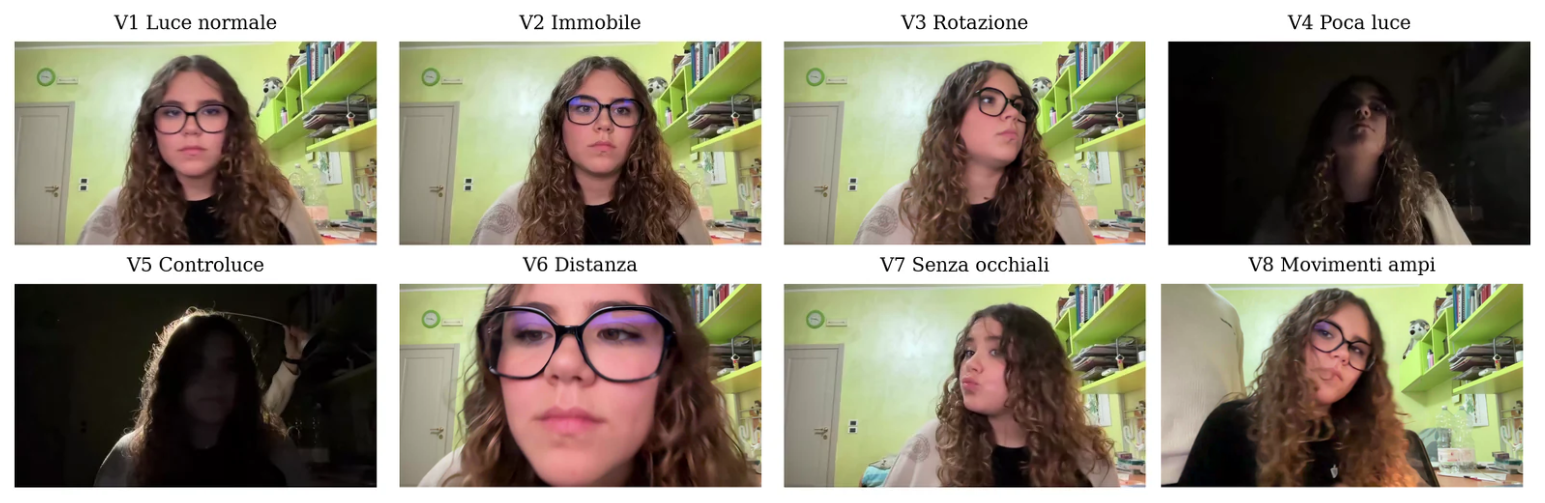
\includegraphics[width=0.9\linewidth]{images/condizioniAcquisizione.png}
    \caption{Condizioni di acquisizione V1-V9 del dataset reale}
    \label{fig:condizioniAcquisizione}
\end{figure}
La \textbf{galleria dei documenti} comprende:
\begin{itemize}
    \item le \gls{cie} dei tre soggetti registrati (due immagini ciascuno per S2 e S3, una delle quali scattata deliberatamente a bassa qualità)
    \item i documenti di cinque persone che non hanno fornito video (quattro \gls{cie} e una patente di guida)
    \item una \gls{cie} sintetica\footnote{Generata con \url{https://github.com/SandroGT/SynthIDGenerator}, che permette di creare documenti realistici a partire da un dataset di immagini ovvero: \url{https://github.com/Raul2718/FLUXSynID}. Esso contiene 14\,889 identità sintetiche, ciascuna con un'immagine frontale in stile documento e alcune immagini \textit{live} della stessa identità, ottenute variando posa, espressione e contesto~\cite{ismayilovFLUXSynIDFrameworkIdentityControlled2025}.} generata artificialmente
    \item due fotografie di S2 e S3 da bambini, usate per una prova di \textit{age-gap}
\end{itemize}
Le immagini sono state scattate con lo smartphone in condizioni \textbf{volutamente eterogenee}: documento dritto o in forte prospettiva, tenuto in mano, con riflessi sul policarbonato, con un dito su un angolo o acquisito con uno scanner piano.
Le identità prive di video svolgono il ruolo di \textbf{impostori}: ogni sessione viene confrontata con l'intera galleria, come avverrebbe nella ricerca $1{:}N$ del sistema reale, per cui ogni finestra di un soggetto genera confronti genuini con le proprie immagini e confronti impostori con tutte le altre.
L'impiego di un \textbf{dataset sintetico} su larga scala è stato valutato e scartato visto che si tratta di immagini singole e non di sequenze video.
Il protocollo di accesso del sistema richiede invece un flusso video di almeno $N$ fotogrammi, in cui la \textit{liveness} e il controllo di staticità osservano proprio la variazione nel tempo.
Animare artificialmente le immagini \textit{live} per ottenerne dei video avrebbe introdotto un movimento sintetico non rappresentativo di una persona reale, e una singola immagine ripetuta verrebbe correttamente bloccata dal controllo di staticità. 
Un dataset di questo tipo avrebbe quindi permesso di valutare solo il confronto tra volto e documento, non la sessione completa.
Per questo motivo si è preferito raccogliere registrazioni reali, meno numerose ma acquisite nelle stesse condizioni d'uso del sistema.
Gli \textbf{attacchi di presentazione} sono stati registrati con lo stesso dispositivo e nella stessa stanza dei video \textit{bona fide}, così da non introdurre differenze dovute alla fotocamera, e sono riassunti nella Tabella~\ref{tab:attacchiDataset}.
Seguendo la terminologia dello standard, ogni strumento di attacco (\gls{pai}) appartiene a una specie: foto stampata (\texttt{PRINT}), riproduzione su schermo (\texttt{SCREEN}) e iniezione tramite fotocamera virtuale, distinta tra video e immagine fissa~\cite{groupBiometricLivenessPresentation}.
\begin{table}[htbp]
    \centering
    \footnotesize
    \renewcommand{\arraystretch}{1.25}
    \begin{tabular*}{0.95\textwidth}{@{\extracolsep{\fill}} l p{0.42\textwidth} c c @{}}
        \hline
        \textbf{Specie} & \textbf{Strumento di attacco} & \textbf{Fotogrammi} & \textbf{Sessioni} \\
        \hline
        \texttt{PRINT} & Foto stampata attuale & 322 & 9 \\
        \texttt{PRINT} & Foto stampata da bambino & 181 & 5 \\
        \texttt{SCREEN} & Foto su smartphone, lontano dalla fotocamera & 124 & 7 \\
        \texttt{SCREEN} & Foto su smartphone, avvicinata e allontanata & 343 & 9 \\
        \texttt{SCREEN} & Video su smartphone, molto vicino e in orizzontale & 323 & 20 \\
        \texttt{SCREEN} & Video su smartphone & 160 & 12 \\
        \texttt{SCREEN} & Video su tablet (iPad) & 260 & 22 \\
        Iniezione video & Video originale inviato tramite OBS\footnotemark \textit{Virtual Camera} & 190 & 5 \\
        Iniezione immagine & Immagine fissa sintetica ripetuta per 10 s & 250 & 7 \\
        \hline
        \multicolumn{2}{@{}l}{\textbf{Totale attacchi}} & 2\,153 & 96 \\
        \hline
    \end{tabular*}
    \caption[Attacchi di presentazione e di iniezione registrati]{Attacchi di presentazione e di iniezione registrati. Tutti gli attacchi sono rivolti all'identità del soggetto S2, tranne l'immagine iniettata, che riproduce l'identità sintetica.}
    \label{tab:attacchiDataset}
\end{table}
\footnotetext{Open Broadcaster Software (OBS) è un software open source per lo streaming e la registrazione video. La fotocamera virtuale permette di inviare al sistema un video pre-registrato come se fosse la webcam.}

\paragraph{Metriche biometriche}
La valutazione del confronto tra volto e documento (Capitolo~\ref{cap:4.2-verifica}) è condotta su \textbf{finestre} di $N = 35$ fotogrammi consecutivi con volto, non sovrapposte.
Da ciascuna finestra si estrae $f_{\text{best}}$ e se ne confronta l'embedding con tutte le immagini della galleria, ottenendo 311 confronti genuini e 1\,834 confronti impostori.
Su queste coppie si calcolano il \gls{far} e il \gls{frr} al variare della soglia $\tau$, come definiti nel Capitolo~\ref{cap:1.1-fondamenti}, la curva \gls{roc} e il punto di equivalenza \gls{err} dell'Equazione~\eqref{eq:eer}.
Alla curva \gls{roc} si affianca la curva \textbf{\gls{det}}, che riporta i due tassi di errore su assi in scala \textit{probit}: in questa scala le differenze tra configurazioni a bassi tassi di errore restano leggibili, e l'intervallo rappresentato è limitato a $[0, 50]\%$~\cite{gonzalezForgedPresentationAttack2025}.
Con 1\,834 confronti impostori il più piccolo \gls{far} non nullo osservabile è circa $0{,}05\%$, limite di cui si terrà conto nell'interpretazione dei risultati.

La valutazione della \textit{liveness} (Capitolo~\ref{cap:4.3-liveness}) è condotta invece sulle intere \textbf{sessioni} simulate.
Per ogni specie di attacco $s$ si calcola l'\gls{apcer} come quota di sessioni di attacco che la \textit{liveness} non riconosce come tali, e si riporta il valore peggiore tra le specie, come descritto nell'Equazione~\eqref{eq:apcerSpecie}~\cite{gonzalezForgedPresentationAttack2025,groupBiometricLivenessPresentation}:
\begin{equation}
    \label{eq:apcerSpecie}
    \text{APCER}_s = \frac{\left|\{\text{sessioni di attacco } s \text{ non classificate come attacco}\}\right|}{\left|\{\text{sessioni di attacco } s\}\right|}
\end{equation}
Poiché il blocco del soggetto immobile è un comportamento voluto, il \gls{bpcer}, invece, è calcolato sulle sessioni in cui il soggetto si muove (condizioni V1 e V3-V9), mentre la condizione V2 è riportata a parte come tasso di blocco per staticità.
Si riporta infine la quota di attacchi accettati dal sistema completo, analoga all'\gls{iapar}, cioè la frazione di sessioni di attacco che si concludono con \texttt{MATCH} sull'identità attaccata~\cite{groupBiometricLivenessPresentation}.

Le \textbf{metriche di sistema} misurano il costo computazionale di ciascuno stadio della pipeline del Capitolo~\ref{cap:2.3-pipeline}, misurati con un orologio ad alta risoluzione e riportati come media, mediana e 95° percentile, insieme al tempo di caricamento dei modelli $T_{\text{load}}$.
Il tempo di una sessione simulata di $N$ fotogrammi è stimato come:
\begin{equation}
    \label{eq:tempoSessioneSimulato}
    T_{\text{sessione}} = \sum_{t=1}^{N} \max\left(\Delta, \; T_{\text{dec}, t} + T_{\text{det}, t} + T_{\text{pad}, t}\right), \qquad \Delta = 40~\text{ms}
\end{equation}
che equivale al tempo minimo imposto dal client finché l'elaborazione del server resta più rapida dell'intervallo di campionamento.

% Ambiente hardware/software (Apple M2); Dataset reale e sintetico; Metriche biometriche e di sistema
% 3pp

\section{Valutazione Face Verification Cross-Domain}\label{cap:4.2-verifica}
Il cuore del sistema è un confronto tra due immagini che non sono mai state pensate per essere confrontate: una fototessera stampata su policarbonato, rifotografata con uno smartphone, e un fotogramma proveniente da una webcam.
Il Capitolo~\ref{cap:1-fondamenti} ha descritto in termini qualitativi perché questo confronto tra domini \textbf{sia più difficile} della verifica tra due fotografie dello stesso tipo.
Si analizzano in questa sezione:
\begin{itemize}
    \item la separabilità dei punteggi
    \item la scelta della soglia $\tau$
    \item l'influenza delle condizioni di acquisizione
    \item l'impatto della pipeline di rettifica della \gls{cie}
    \item il confronto tra i due pacchetti di modelli di InsightFace (\texttt{buffalo\_l} e \texttt{buffalo\_s})
    \item l'impatto della risoluzione del rilevatore di volti
\end{itemize}

\paragraph{Separabilità dei punteggi}
La Figura~\ref{fig:distribuzioniGenuiniImpostori} mostra le distribuzioni della similarità coseno ottenute con la configurazione del server (\texttt{buffalo\_l}, rilevatore a $320 \times 320$ pixel, \gls{cie} rettificata ed equalizzata con \gls{clahe}) sulle finestre di $N = 35$ fotogrammi.
I confronti \textbf{impostori} si concentrano attorno allo zero, con media $0{,}060$ e deviazione standard $0{,}090$, come ci si attende da embedding di identità diverse distribuiti quasi ortogonalmente sull'ipersfera.
I confronti \textbf{genuini} hanno invece media $0{,}356$ e deviazione standard $0{,}063$: le due distribuzioni sono ben separate, ma il centro della distribuzione genuina è molto più basso dei valori tipici della verifica tra due fotografie dello stesso dominio, e lontano dall'intervallo $\tau \in [0{,}50, 0{,}60]$ indicato nel Capitolo~\ref{cap:1.1-fondamenti} per i modelli basati su ArcFace.
Il punto di equivalenza si trova a $\tau = 0{,}23$, con un \gls{err} del $4{,}8\%$.

\begin{figure}[H]
    \centering
    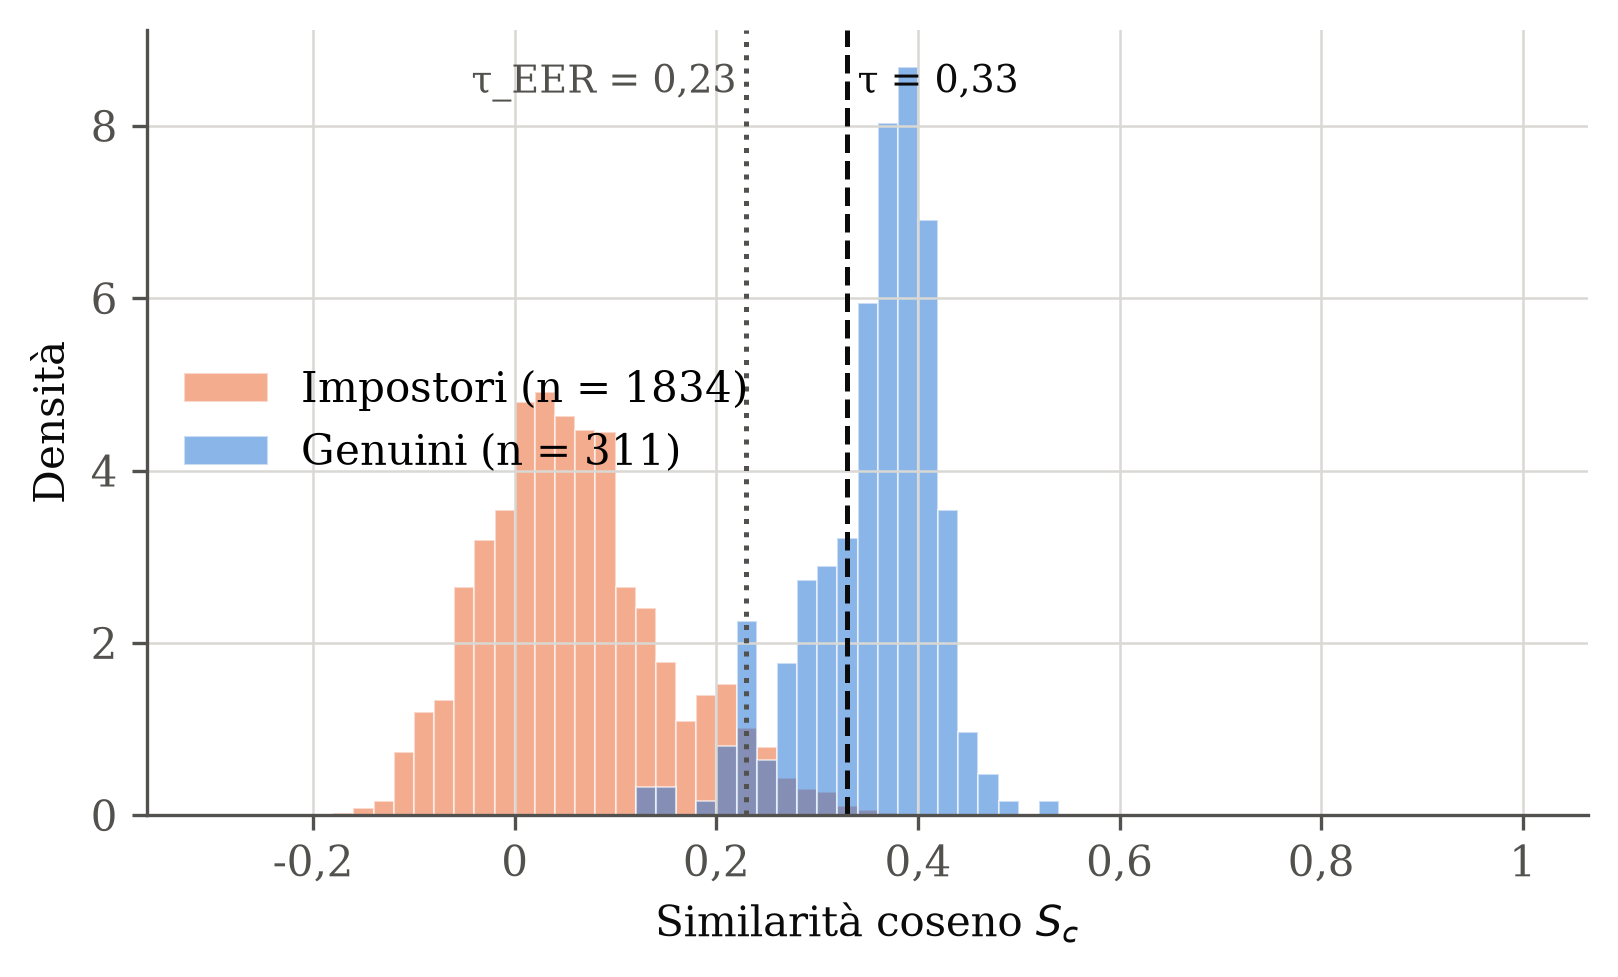
\includegraphics[width=0.85\linewidth]{images/distribuzioniGenuiniImpostori.png}
    \caption[Distribuzioni della similarità coseno tra volto e documento]{Distribuzioni della similarità coseno $S_c$ tra il fotogramma $f_{\text{best}}$ di ogni finestra e le immagini della galleria. La linea tratteggiata indica la soglia adottata, quella punteggiata la soglia di equivalenza.}
    \label{fig:distribuzioniGenuiniImpostori}
\end{figure}

Il valore basso dei punteggi genuini è coerente con quanto osservato in letteratura per il confronto tra documento e selfie, dove le difficoltà principali non derivano tanto da posa o espressione, quanto dalla bassa qualità della fototessera e dal tempo trascorso dal rilascio del documento~\cite{shiDocFaceMatchingID2018}.
Modelli generici che superano il 92\% di \gls{tar} a $\text{FAR} = 0{,}1\%$ su immagini dello stesso dominio scendono tra il 46\% e il 61\% su coppie documento-selfie, e solo un modello addestrato specificamente su questo tipo di coppie raggiunge il 92,8\%~\cite{shiDocFaceMatchingID2018}.
Sul dataset raccolto, \texttt{buffalo\_l} raggiunge un \gls{tar} del 65,6\% a $\text{FAR} = 0{,}1\%$ e dell'82,0\% a $\text{FAR} = 1\%$.

La coda alta della distribuzione impostori ha un'origine precisa: sei confronti impostori superano la soglia $\tau = 0{,}33$, e cinque di essi riguardano la \textbf{coppia di fratelli} S2 e S3.
Le finestre di S3 confrontate con la \gls{cie} di S2 raggiungono una similarità media di $0{,}242$ e massima di $0{,}347$, quelle di S2 confrontate con la \gls{cie} di S3 una media di $0{,}187$.
Escludendo questa coppia, la media degli impostori scende a $0{,}037$.
Si tratta dello stesso fenomeno descritto da \textit{DocFace}, dove i falsi accettati si concentrano tra impostori molto simili, resi ancora più difficili da distinguere dalla bassa qualità della foto del documento~\cite{shiDocFaceMatchingID2018}.
Nella ricerca $1{:}N$ questo effetto resta contenuto: tra le 198 sessioni che superano la \textit{liveness}, il primo risultato appartiene al soggetto corretto nel 96,5\% dei casi, e \textbf{una sola sessione} produce un \texttt{MATCH} con l'identità sbagliata.
\paragraph{Scelta della soglia $\tau$}
La soglia $\tau = 0{,}35$ inizialmente fissata nella configurazione (Tabella~\ref{tab:env}) si è rivelata \textbf{troppo severa} per questo scenario.
La Tabella~\ref{tab:sogliaSimilarita} riporta, al variare di $\tau$, i tassi di errore misurati sulle finestre e due grandezze misurate sulle sessioni complete: la quota di sessioni \textit{bona fide} in movimento che si concludono con un \texttt{MATCH} corretto e la quota di sessioni di attacco accettate dal sistema.
Questa seconda grandezza è decisiva, perché alcuni attacchi superano la \textit{liveness} (Capitolo~\ref{cap:4.3-liveness}) e vengono fermati soltanto dal confronto con il documento.

\begin{table}[htbp]
    \centering
    \footnotesize
    \renewcommand{\arraystretch}{1.25}
    \begin{tabular*}{\textwidth}{@{\extracolsep{\fill}}ccccc@{}}
        \hline
        \textbf{Soglia $\tau$} & \textbf{\gls{far}} & \textbf{\gls{frr}} & \textbf{Bona fide accettate} & \textbf{Attacchi accettati} \\
        \hline
        $0{,}23$ & $4{,}7\%$ & $4{,}8\%$ & $87{,}3\%$ & $28{,}1\%$ \\
        $0{,}25$ & $3{,}1\%$ & $9{,}0\%$ & $85{,}5\%$ & $24{,}0\%$ \\
        $0{,}28$ & $1{,}5\%$ & $12{,}5\%$ & $82{,}7\%$ & $19{,}8\%$ \\
        $0{,}30$ & $0{,}9\%$ & $18{,}0\%$ & $77{,}5\%$ & $14{,}6\%$ \\
        $\mathbf{0{,}33}$ & $\mathbf{0{,}3\%}$ & $\mathbf{26{,}7\%}$ & $\mathbf{69{,}9\%}$ & $\mathbf{8{,}3\%}$ \\
        $0{,}35$ & $0{,}05\%$ & $36{,}3\%$ & $60{,}1\%$ & $4{,}2\%$ \\
        $0{,}40$ & $0\%$ & $75{,}6\%$ & $24{,}3\%$ & $0\%$ \\
        \hline
    \end{tabular*}
    \caption[Effetto della soglia di similarità]{Effetto della soglia di similarità. Le sessioni \textit{bona fide} accettate sono quelle concluse con \texttt{MATCH} sull'identità corretta. Gli attacchi accettati sono le sessioni di attacco concluse con \texttt{MATCH} sull'identità attaccata.}
    \label{tab:sogliaSimilarita}
\end{table}
La scelta della soglia dipende dal profilo di rischio del servizio: i percorsi ad alto rischio, come l'apertura di un conto o il recupero di un account, richiedono soglie severe anche a costo di una maggiore frizione per l'utente~\cite{groupBiometricLivenessPresentation}.
Abbassare la soglia fino al punto di equivalenza renderebbe il sistema molto più comodo, ma lascerebbe entrare più di un attacco su quattro.
Si è scelto quindi di adottare la soglia $\tau = 0{,}33$.

\paragraph{Influenza delle condizioni di acquisizione}
La Figura~\ref{fig:genuiniPerCondizione} scompone i punteggi genuini per condizione di acquisizione.
Nelle condizioni di riferimento la verifica è quasi sempre corretta: con luce normale il \gls{frr} è del 2,8\%, invece con poca luce il \gls{frr} sale al 52,6\% e in controluce al 57,1\%, con una similarità media che scende da $0{,}38$ a circa $0{,}31$.
Anche la condizione senza occhiali presenta un \gls{frr} elevato (45,2\%) e le espressioni accentuate e i movimenti ampi del corpo si collocano in posizione intermedia, con un \gls{frr} tra il 20\% e il 28\%.

\begin{figure}[H]
    \centering
    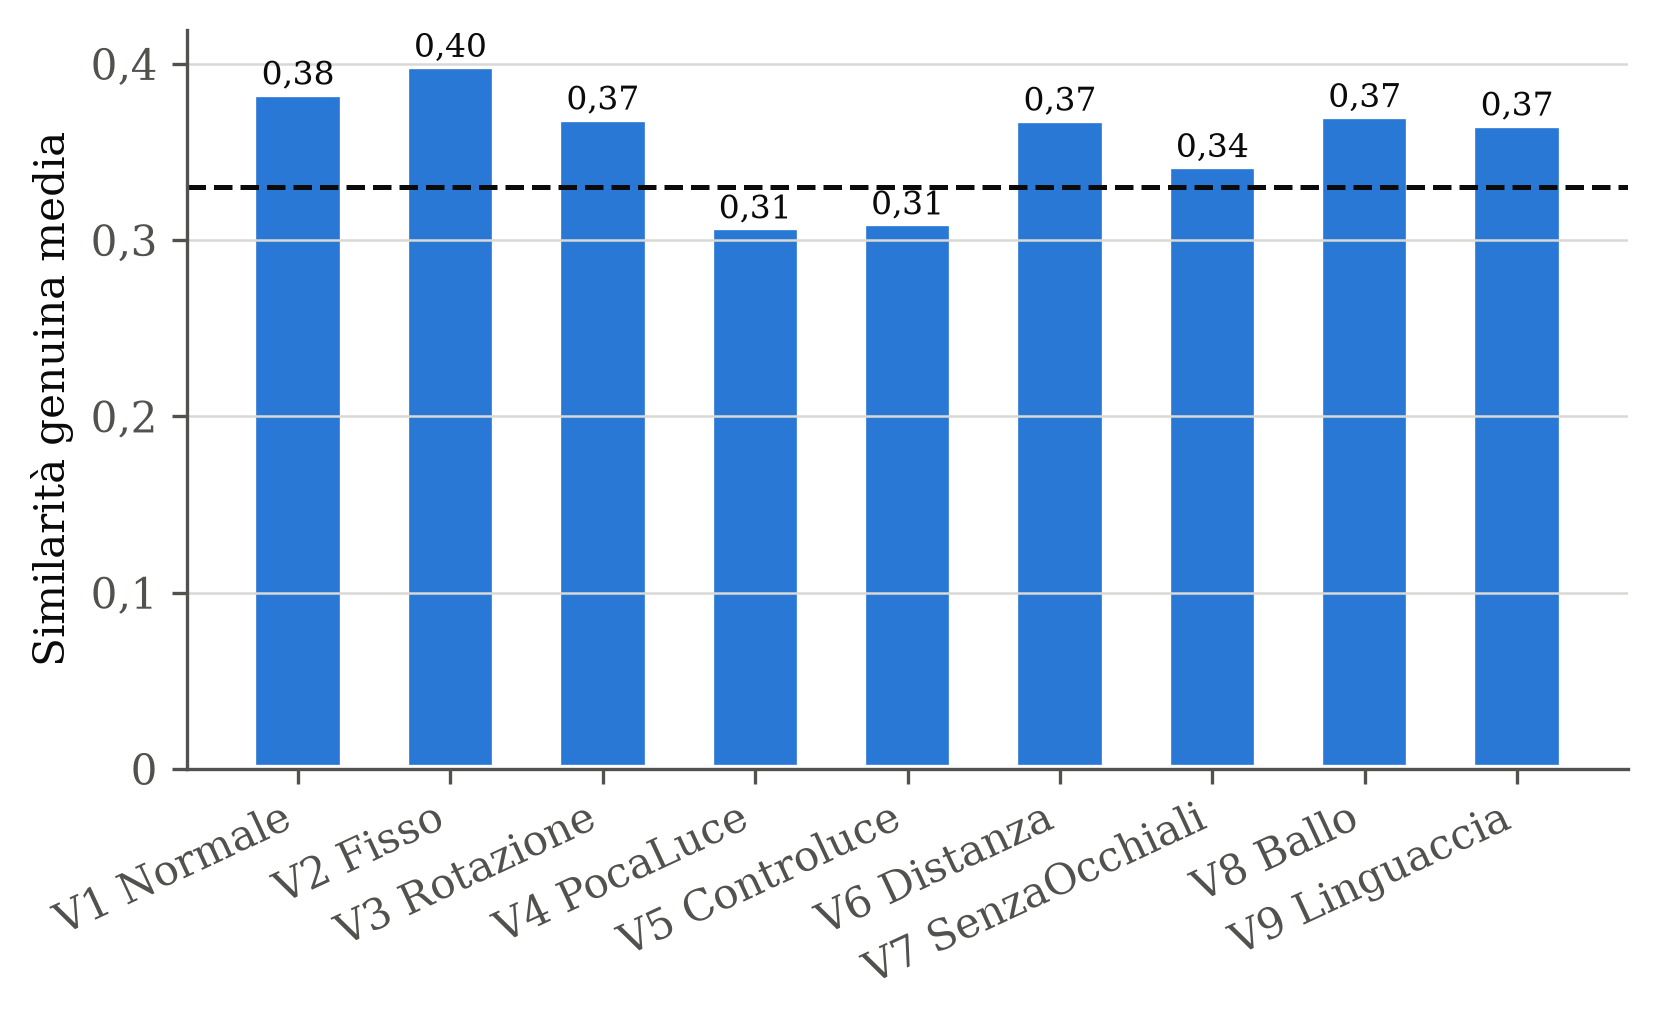
\includegraphics[width=0.85\linewidth]{images/genuiniPerCondizione.png}
    \caption[Similarità genuina media per condizione di acquisizione]{Similarità genuina media per condizione di acquisizione. La linea tratteggiata indica la soglia $\tau = 0{,}33$.}
    \label{fig:genuiniPerCondizione}
\end{figure}
Una prova aggiuntiva riguarda l'\textit{age-gap}, cioè la distanza temporale tra l'immagine di riferimento e il volto attuale.
Usando come riferimento una fotografia dei soggetti da bambini al posto della \gls{cie}, la similarità media con i video attuali è $0{,}30$ per S2 e $0{,}33$ per S3, contro $0{,}34$ e $0{,}37$ ottenuti con il documento.
Confrontando invece la foto da bambino direttamente con la \gls{cie} attuale, S2 ottiene $0{,}32$ e S3 $0{,}10$.
Il modello conserva quindi una parte dell'informazione identitaria anche a distanza di molti anni, ma in modo \textbf{troppo irregolare} per essere affidabile: la differenza d'età resta uno dei fattori che spiegano i falsi rifiuti nel confronto con documenti rilasciati da tempo~\cite{shiDocFaceMatchingID2018}.

\paragraph{Impatto della pipeline di rettifica della \gls{cie}}
Per valutare il contributo delle singole fasi di pre-elaborazione, la Tabella~\ref{tab:ablationCIE} confronta, sugli stessi video, quattro varianti della galleria: immagine grezza, solo \gls{clahe}, solo rettifica prospettica e rettifica seguita da \gls{clahe}, che è la configurazione del sistema.
Il risultato più netto riguarda il \textbf{rilevamento}: senza rettifica il volto viene trovato solo nel 73\% delle immagini di documento, perché la fototessera occupa una porzione troppo piccola dello scatto o è deformata dalla prospettiva, mentre con la rettifica viene trovato nel 100\% dei casi.
La rettifica \textbf{è riuscita} in dieci immagini su undici: l'unico fallimento riguarda un documento tenuto in mano, per il quale il quadrilatero non soddisfa i vincoli geometrici e il sistema prosegue con l'immagine non rettificata, rilevando comunque il volto.

\begin{table}[htbp]
    \centering
    \footnotesize
    \renewcommand{\arraystretch}{1.25}
    \begin{tabular*}{\textwidth}{@{\extracolsep{\fill}}lccccc@{}}
        \hline
        \textbf{Variante} & \textbf{Volto rilevato} & \textbf{Media genuini} & \textbf{\gls{err}} & \textbf{\gls{far}} & \textbf{\gls{frr}} \\
        \hline
        Grezza & $73\%$ & $0{,}361$ & $6{,}6\%$ & $0{,}51\%$ & $31{,}7\%$ \\
        Solo \gls{clahe} & $73\%$ & $0{,}357$ & $4{,}9\%$ & $0{,}07\%$ & $32{,}2\%$ \\
        Solo rettifica & $100\%$ & $0{,}362$ & $4{,}6\%$ & $0{,}33\%$ & $26{,}0\%$ \\
        Rettifica + \gls{clahe} & $100\%$ & $0{,}356$ & $4{,}8\%$ & $0{,}33\%$ & $26{,}7\%$ \\
        \hline
    \end{tabular*}
    \caption{Valutazione delle prestazioni mediante disattivazione progressiva dei moduli della pipeline di rettifica del documento. }
    \label{tab:ablationCIE}
\end{table}

Sui punteggi la rettifica riduce l'\gls{err} dal 6,6\% al 4,6\% come mostrano le curve \gls{roc} e \gls{det} della Figura~\ref{fig:rocDetAblation}, dove la variante grezza è l'unica a staccarsi nettamente dalle altre.
Il contributo di \gls{clahe} \textbf{è invece marginale} e non sistematico: migliora l'\gls{err} quando è applicato da solo, mentre in combinazione con la rettifica lascia i tassi di errore sostanzialmente invariati.

\begin{figure}[H]
    \centering
    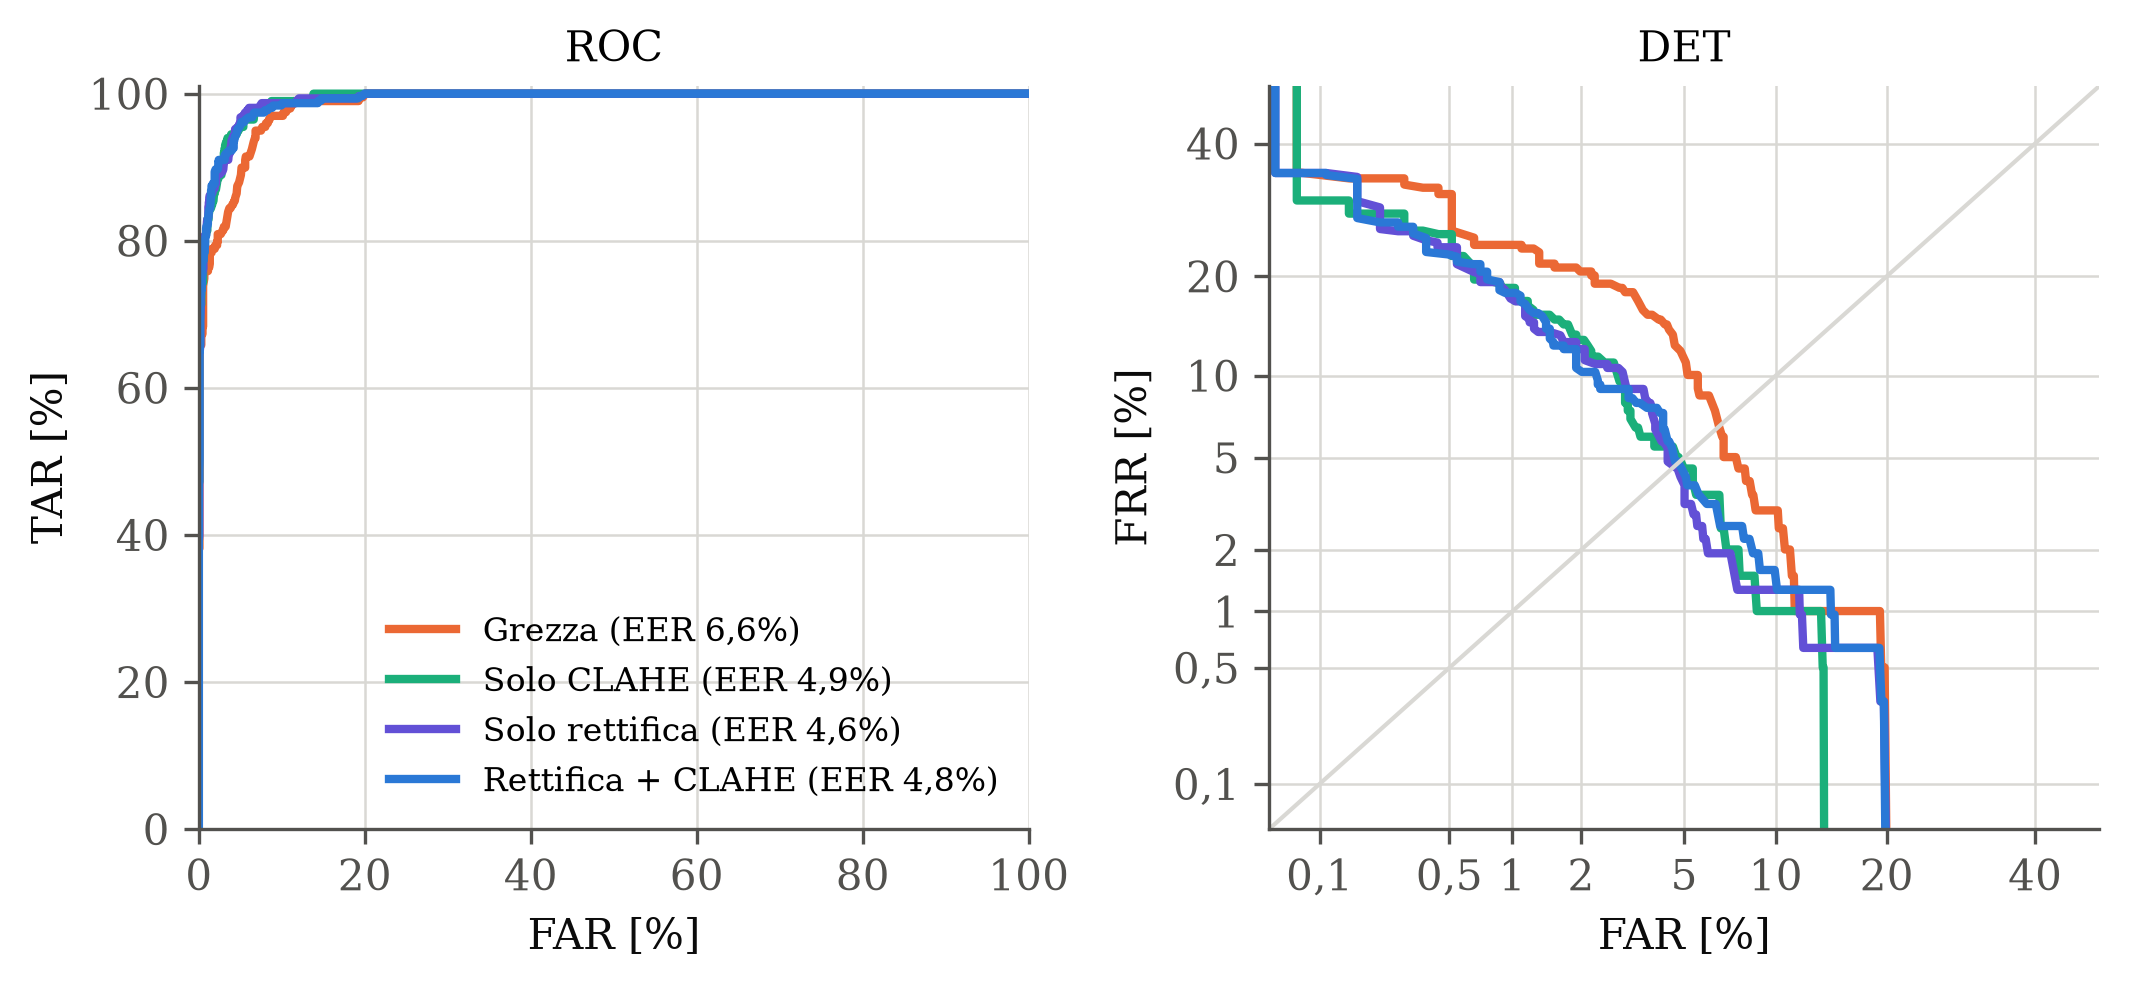
\includegraphics[width=\linewidth]{images/rocDetAblation.png}
    \caption[Curve ROC e DET dello studio di ablazione sul documento]{Curve \gls{roc} (a sinistra) e \gls{det} (a destra, assi in scala \textit{probit}) per le quattro varianti di pre-elaborazione del documento.}
    \label{fig:rocDetAblation}
\end{figure}

\paragraph{Confronto tra modelli e risoluzioni del rilevatore}
I risultati sono riassunti nella Tabella~\ref{tab:confrontoModelli}.
\begin{table}[htbp]
    \centering
    \footnotesize
    \renewcommand{\arraystretch}{1.25}
    \begin{tabular*}{\textwidth}{@{\extracolsep{\fill}}lccccc@{}}
        \hline
        \textbf{Configurazione} & \textbf{Volto rilevato} & \textbf{Media genuini} & \textbf{\gls{err}} & \textbf{$T_{\text{det}}$ [ms]} & \textbf{$T_{\text{emb}}$ [ms]} \\
        \hline
        \texttt{buffalo\_l}, rilevatore 160 & $94{,}7\%$ & $0{,}361$ & $4{,}7\%$ & $6{,}8$ & $3{,}8$ \\
        \texttt{buffalo\_l}, rilevatore 320 & $97{,}8\%$ & $0{,}356$ & $4{,}8\%$ & $12{,}0$ & $3{,}9$ \\
        \texttt{buffalo\_l}, rilevatore 640 & $97{,}0\%$ & $0{,}367$ & $4{,}7\%$ & $21{,}1$ & $4{,}0$ \\
        \texttt{buffalo\_sc}, rilevatore 320 & $96{,}3\%$ & $0{,}287$ & $10{,}4\%$ & $4{,}7$ & $1{,}3$ \\
        \hline
    \end{tabular*}
    \caption[Confronto tra pacchetti di modelli e risoluzioni del rilevatore]{Confronto tra pacchetti di modelli e risoluzioni del rilevatore sugli stessi video. I tempi sono medie per fotogramma con il provider \textit{CoreML}.}
    \label{tab:confrontoModelli}
\end{table}
La risoluzione del rilevatore incide sulla capacità di trovare il volto più che sulla qualità del confronto.
Dimezzarla a $160 \times 160$ pixel quasi dimezza il tempo di rilevamento, ma il volto viene perso nel 5,3\% dei fotogrammi, contro il 2,2\% della configurazione a $320 \times 320$ pixel.
Una volta trovato il volto, però, l'\gls{err} resta invariato, perché l'allineamento e l'embedding lavorano comunque sul ritaglio dell'immagine originale.
Raddoppiarla a $640 \times 640$ pixel \textbf{non porta alcun beneficio} misurabile e quasi raddoppia il tempo di rilevamento.
Il pacchetto \texttt{buffalo\_sc} è il più rapido, con un costo complessivo di circa 6~ms per fotogramma, ma la media dei punteggi genuini scende a $0{,}287$ e l'\gls{err} raddoppia, passando dal 4,8\% al 10,4\%: la rete più leggera separa peggio le identità proprio nello scenario in cui il margine tra genuini e impostori è già ridotto.
La configurazione adottata dal server, \texttt{buffalo\_l} con rilevatore a $320 \times 320$ pixel, risulta quindi il compromesso migliore tra i quattro.

% Separabilità genuine/impostor, curve ROC/DET ed EER, Ablation study sul preprocessing CIE e confronto buffaloL vs buffaloSc
% 5pp

\section{Valutazione della Liveness Detection e delle prestazioni}\label{cap:4.3-liveness}
Un confronto tra volto e documento affidabile non serve a nulla se chiunque può presentare alla fotocamera la fotografia di un altro: la verifica di vitalità è ciò che trasforma un sistema di riconoscimento in un \textbf{sistema di autenticazione}.
Valutiamo quindi la difesa a più livelli costruita nei capitoli precedenti e i relativi costi, cioè:
\begin{itemize}
    \item la classificazione di \textit{MiniFASNet} sui singoli fotogrammi
    \item il controllo di staticità del soggetto
    \item l'influenza della lunghezza del buffer
    \item la durata della sessione
    \item la latenza di ciascuno stadio
    \item l'occupazione di memoria e CPU sul dispositivo
\end{itemize}
\paragraph{Rilevamento degli attacchi di presentazione (\gls{pa})}
La Tabella~\ref{tab:attacchiPerPai} riassume l'esito delle 96 sessioni di attacco simulate con la configurazione del server.
Per ogni tipologia sono riportati due valori distinti: l'\gls{apcer}, cioè la quota di sessioni che superano i controlli di vitalità, e la quota di sessioni accettate dal sistema completo.
Mantenere separate le due grandezze è necessario per non valutare il modulo \gls{pad} da solo, visto che un attaccante è interessato soltanto al risultato finale~\cite{groupBiometricLivenessPresentation}.

\begin{table}[htbp]
    \centering
    \footnotesize
    \renewcommand{\arraystretch}{1.25}
    \begin{tabular*}{\textwidth}{@{\extracolsep{\fill}}lcccc@{}}
        \hline
        \textbf{Tipo di attacco} & \textbf{Video} & \textbf{Sessioni} & \textbf{Liveness (\gls{apcer})} & \textbf{Accettati} \\
        \hline
        \texttt{SCREEN} (smartphone e tablet) & 5 & 70 & $18{,}6\%$ & $10{,}0\%$ \\
        \texttt{PRINT} (foto stampata) & 2 & 14 & $92{,}9\%$ & $0\%$ \\
        Iniezione video & 1 & 5 & $100\%$ & $20{,}0\%$ \\
        Iniezione immagine fissa & 1 & 7 & $0\%$ & $0\%$ \\
        \hline
        \multicolumn{3}{@{}l}{\textbf{Caso peggiore (presentazione al sensore)}} & $92{,}9\%$ & $10{,}0\%$ \\
        \hline
    \end{tabular*}
    \caption[Esito delle sessioni di attacco per tipologia]{Esito delle sessioni di attacco per tipologia ($N = 35$, $M = 7$, $\tau_{\text{liveness}} = 0{,}60$, $\tau_{\text{static}} = 0{,}005$, $\tau = 0{,}33$). Gli attacchi accettati dal sistema sono le sessioni concluse con \texttt{MATCH} sull'identità attaccata.}
    \label{tab:attacchiPerPai}
\end{table}
Gli attacchi tramite \textbf{schermo} sono quelli che \textit{MiniFASNet} riconosce meglio: delle 70 sessioni, 57 sono interrotte come attacco, quasi sempre in anticipo per il superamento del contatore $M$, in media dopo meno di \textbf{0,6~secondi}.
Fa eccezione la fotografia mostrata sullo smartphone e avvicinata progressivamente alla fotocamera, che supera la \textit{liveness} in tutte le nove sessioni e ottiene il \texttt{MATCH} in sei\footnote{Una spiegazione plausibile, è che quando lo schermo riempie l'inquadratura i suoi bordi e il contesto circostante escano dal ritaglio analizzato.}.
Questa variabilità all'interno della stessa specie è coerente con la letteratura, dove gli attacchi tramite schermo risultano i più difficili proprio per l'eterogeneità delle risoluzioni e delle distanze di presentazione~\cite{gonzalezForgedPresentationAttack2025}.
Le \textbf{foto stampate} costituiscono il caso peggiore per il modulo \gls{pad}: superano i controlli in 13 sessioni su 14, come mostra la Figura~\ref{fig:pRealPerCondizione}.
Nonostante ciò, nessuna sessione si conclude con un \texttt{MATCH}: la stampa su carta degrada il volto al punto che la similarità con il documento non supera $0{,}31$, sotto la soglia adottata.
Si tratta quindi di una \textbf{protezione fragile}, che dipende dalla qualità della stampa e dalla soglia $\tau$ (Tabella~\ref{tab:sogliaSimilarita}).

\begin{figure}[H]
    \centering
    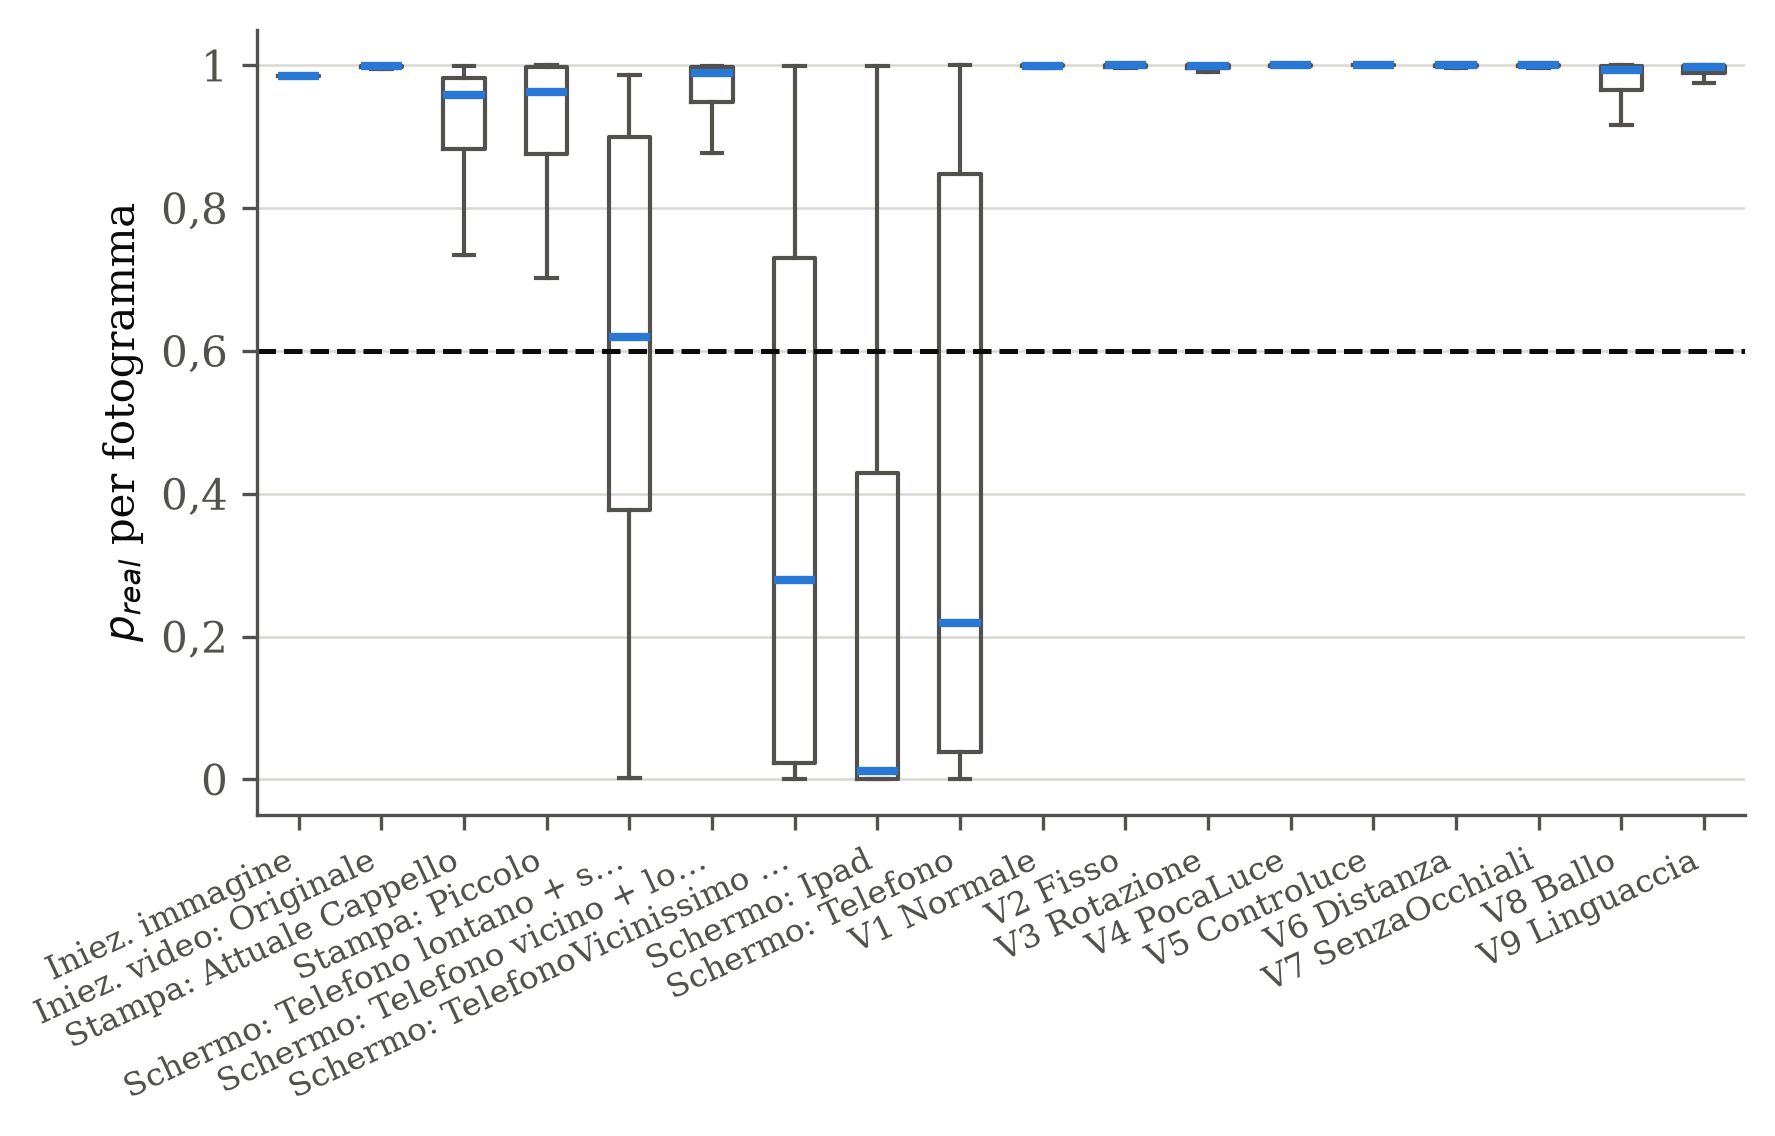
\includegraphics[width=0.9\linewidth]{images/pRealPerCondizione.png}
    \caption[Probabilità di vitalità per fotogramma per condizione]{Distribuzione della probabilità di vitalità $p_{\text{real}}$ stimata da \textit{MiniFASNet} per fotogramma, per ciascun attacco e condizione \textit{bona fide}. La linea tratteggiata indica $\tau_{\text{liveness}} = 0{,}60$.}
    \label{fig:pRealPerCondizione}
\end{figure}
Negli attacchi per \textbf{iniezione} il video originale inviato tramite fotocamera virtuale è, dal punto di vista del server, indistinguibile da una sessione legittima: supera la \textit{liveness} in tutte le sessioni ed è fermato solo dalla similarità, che oscilla attorno alla soglia, con un \texttt{MATCH} su cinque sessioni.
L'immagine fissa iniettata ottiene anch'essa probabilità di vitalità elevate, ma il suo indice di movimento è nullo ($\sigma_{\text{kps}} \approx 0$) e il \textbf{controllo di staticità} la blocca in tutte le sessioni.
Il controllo di staticità si rivela quindi efficace contro l'unico attacco che \textit{MiniFASNet} non vede e che non si muove, ma non può nulla contro un video iniettato, contro il quale le contromisure sarebbero: attestazione del client o rilevamento delle fotocamere virtuali~\cite{groupBiometricLivenessPresentation}.

Sul fronte degli utenti legittimi, delle 173 sessioni in movimento solo 8 vengono classificate come attacco, per un \gls{bpcer} del $4{,}6\%$.
Sette di questi rifiuti sono dovuti al controllo di staticità, in finestre in cui il soggetto si muoveva pochissimo, infatti nella condizione V2, l'88,2\% delle sessioni viene bloccato con \texttt{STATIC\_FACE}.
Il modello di vitalità, quindi produce un \gls{bpcer} \textbf{inferiore all'1\%} anche in condizioni di poca luce e in controluce.

\paragraph{Controllo di staticità}
La Figura~\ref{fig:sigmaKpsPerCondizione} riporta l'indice di movimento $\sigma_{\text{kps}}$, calcolato a partire dal rapporto dell'Equazione~\eqref{eq:rapportoYaw}, su ogni finestra di 35 fotogrammi.
Le condizioni in cui il soggetto si muove liberamente producono valori tra $10^{-2}$ e $10^{-1}$, con la rotazione della testa che raggiunge il massimo.
Il soggetto immobile, invece, si colloca un ordine di grandezza più in basso, con una mediana di $0{,}0019$ e l'immagine iniettata ha correttamente un indice nullo.
Gli attacchi tenuti in mano, stampati o su schermo, hanno \textbf{valori simili a quelli di un utente reale}, perché la mano trasmette al volto riprodotto un movimento continuo. Quindi, il controllo di staticità, da solo, non li distingue.

\begin{figure}[H]
    \centering
    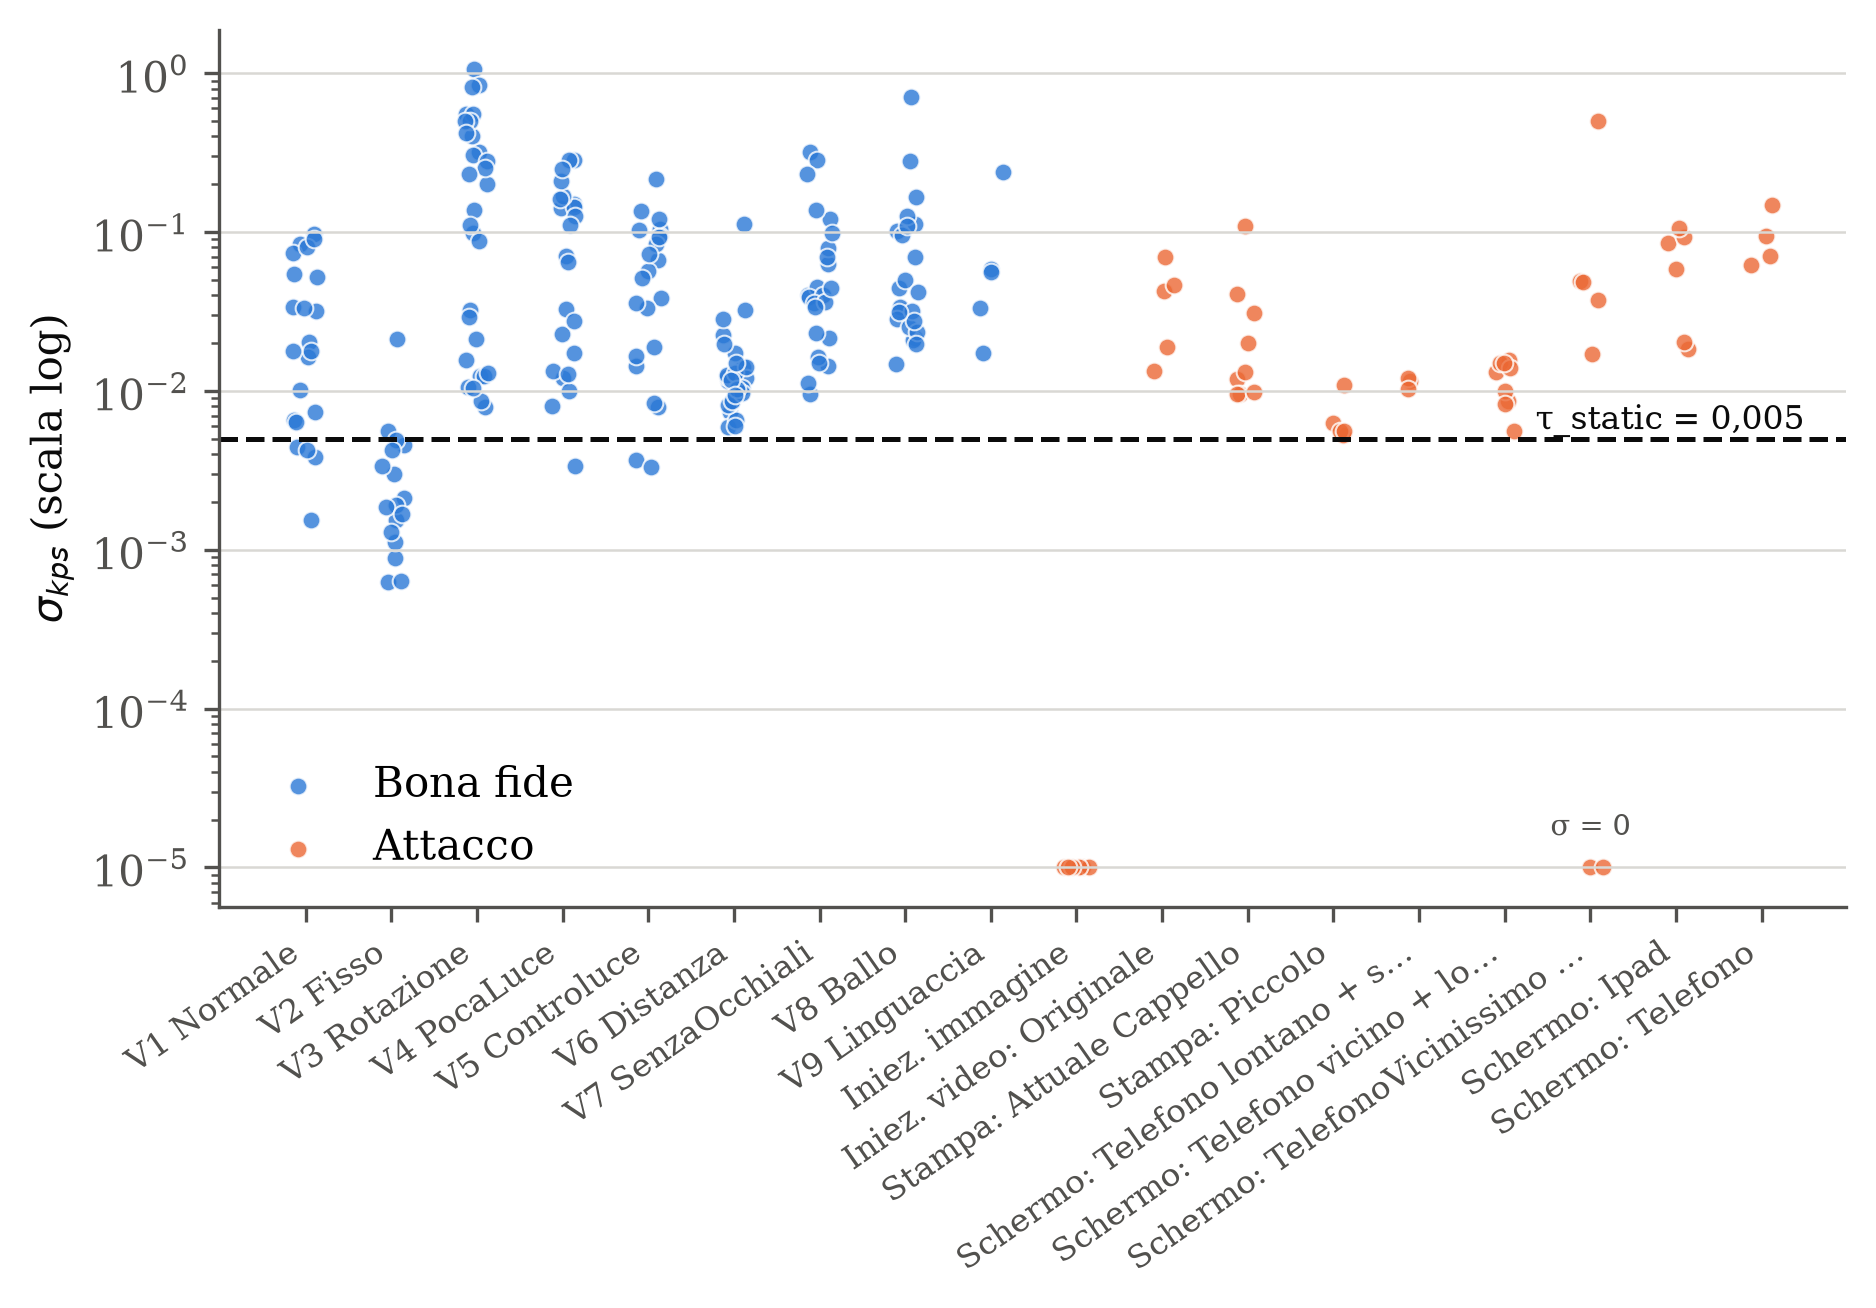
\includegraphics[width=0.95\linewidth]{images/sigmaKpsPerCondizione.png}
    \caption[Indice di movimento per condizione]{Indice di movimento $\sigma_{\text{kps}}$ per la finestra di 35 fotogrammi, per le condizioni \textit{bona fide} (in blu) e per gli attacchi (in arancione). La linea tratteggiata indica $\tau_{\text{static}} = 0{,}005$.}
    \label{fig:sigmaKpsPerCondizione}
\end{figure}

La soglia $\tau_{\text{static}}$ è stata tarata con l'obiettivo esplicito di bloccare chi resta immobile davanti alla fotocamera.
Le due distribuzioni, però, si sovrappongono parzialmente.
La Figura~\ref{fig:sogliaStatica} mostra il compromesso che ne deriva.
\begin{itemize}
    \item Con $\tau_{\text{static}} = 0{,}0005$ nessuna finestra \textit{bona fide} viene bloccata, ma nemmeno quelle del soggetto immobile;
    \item con $0{,}003$ viene bloccato il 58,8\% delle finestre immobili e lo 0,6\% di quelle in movimento
    \item con il valore adottato, $0{,}005$, la quota sale all'88,2\% per le finestre immobili e al 3,9\% per quelle in movimento, concentrate nella condizione normale
    \item Oltre $0{,}0075$ il blocco del soggetto immobile non aumenta più, mentre i falsi blocchi dei soggetti in movimento crescono rapidamente, fino al 14,6\% a $0{,}01$.
\end{itemize}
L'immagine iniettata resta bloccata al 100\% con qualunque soglia.
\begin{figure}[H]
    \centering
    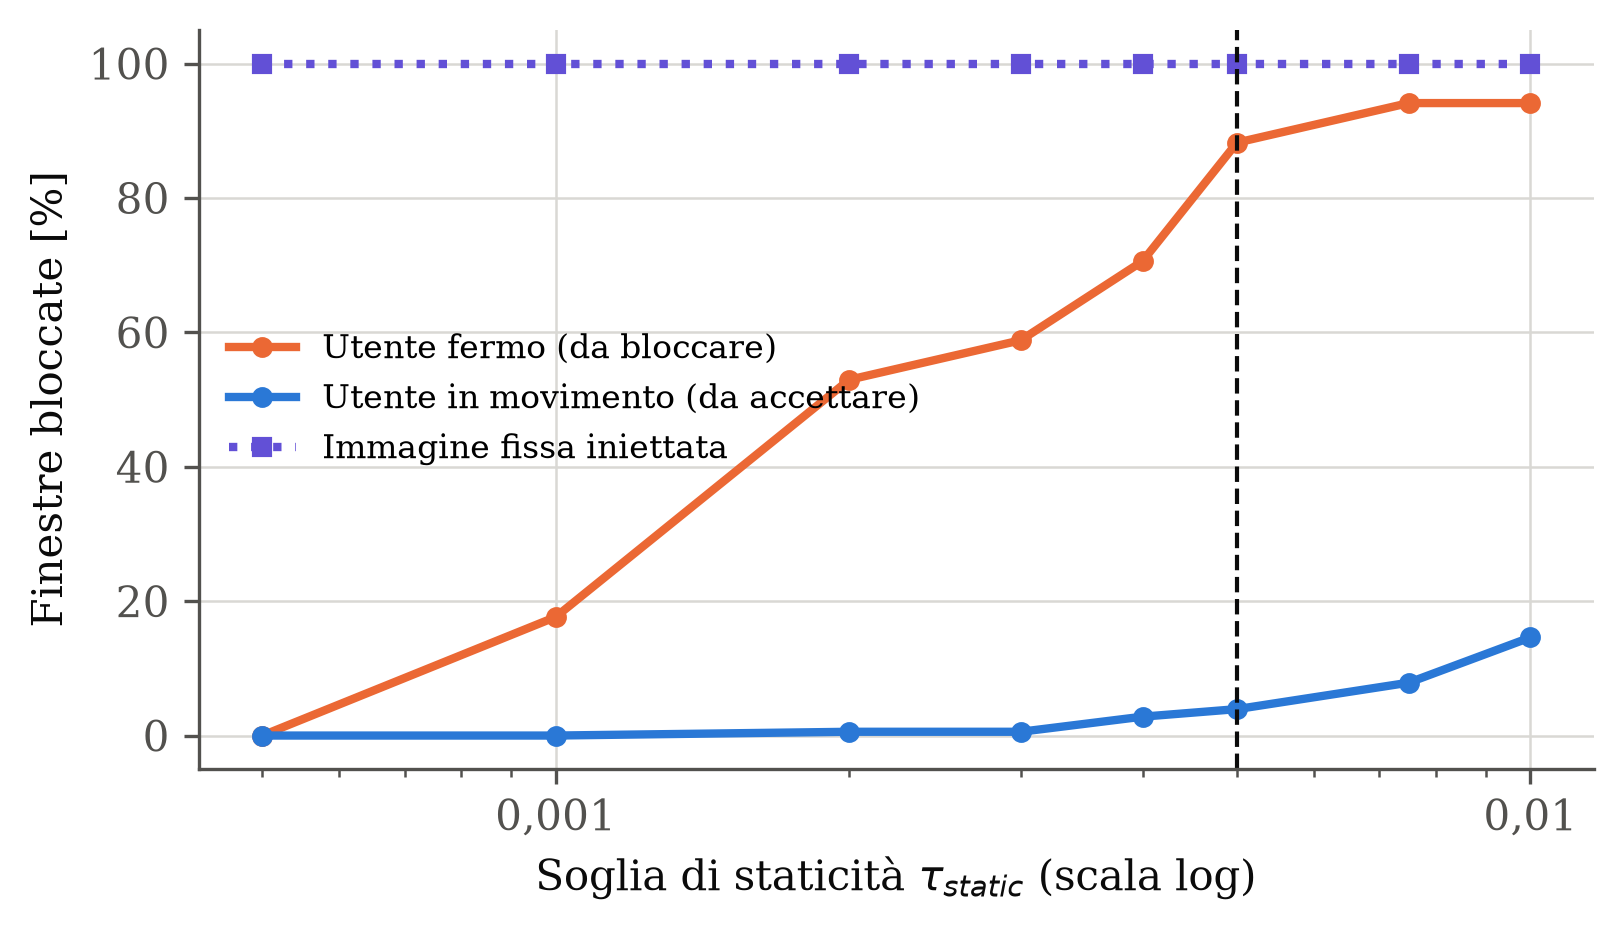
\includegraphics[width=0.8\linewidth]{images/sogliaStatica.png}
    \caption[Taratura della soglia di staticità]{Quota di finestre classificate come statiche al variare di $\tau_{\text{static}}$, per il soggetto immobile (condizione V2), per i soggetti in movimento (V1, V3-V9) e per l'immagine fissa iniettata. La linea tratteggiata indica il valore adottato.}
    \label{fig:sogliaStatica}
\end{figure}

\paragraph{Lunghezza del buffer $N$}
La Tabella~\ref{tab:lunghezzaBuffer} riporta, per cinque valori di $N$, il \gls{bpcer} sulle sessioni in movimento, il blocco del soggetto immobile, l'\gls{apcer} delle due specie presentate al sensore e la durata media di una sessione legittima.
\textbf{Allungare il buffer migliora} entrambi i tassi di errore principali, come mostra la tabella~\ref{tab:lunghezzaBuffer}.
Per gli attacchi su schermo, un buffer più lungo offre più fotogrammi per accumulare segnalazioni e superare il contatore $M$, che resta fisso a 7.
Per gli utenti legittimi, una finestra più lunga contiene più movimento spontaneo, per cui i falsi blocchi per staticità diminuiscono.
Il blocco del soggetto immobile resta invece elevato per tutti i valori, tra il 78\% e il 95\%, mentre il tipo di attacco \texttt{PRINT} supera la \textit{liveness} con qualunque lunghezza del buffer, a conferma che il suo limite è nel modello e non nell'aggregazione.
Il costo è la durata della sessione, che cresce linearmente da circa 0,6 a 2,5~secondi, perché è determinata dall'intervallo di campionamento del client e non dall'elaborazione del server.
Il valore adottato, $N = 35$, \textbf{è un compromesso} tra i due effetti: rispetto a $N = 60$ dimezza l'attesa al prezzo di un \gls{bpcer} e di un \gls{apcer} su schermo più alti rispettivamente di circa 2,5 e 11 punti percentuali.
La sessione dura in media $1{,}45$~secondi, in linea con la durata minima di circa 1,4~secondi prevista nel Capitolo~\ref{cap:3.4-ui}.
\begin{table}[htbp]
    \centering
    \footnotesize
    \renewcommand{\arraystretch}{1.25}
    \begin{tabular*}{\textwidth}{@{\extracolsep{\fill}}cccccc@{}}
        \hline
        \textbf{$N$} & \textbf{\gls{bpcer}} & \textbf{Immobile bloccato} & \textbf{\gls{apcer} \texttt{SCREEN}} & \textbf{\gls{apcer} \texttt{PRINT}} & \textbf{$T_{\text{sessione}}$ [s]} \\
        \hline
        15 & $11{,}9\%$ & $95{,}2\%$ & $35{,}9\%$ & $66{,}7\%$ & $0{,}62$ \\
        25 & $7{,}7\%$ & $88{,}0\%$ & $25{,}0\%$ & $75{,}0\%$ & $1{,}04$ \\
        \textbf{35} & $\mathbf{4{,}6\%}$ & $\mathbf{88{,}2\%}$ & $\mathbf{18{,}6\%}$ & $\mathbf{92{,}9\%}$ & $\mathbf{1{,}45}$ \\
        45 & $3{,}1\%$ & $92{,}9\%$ & $11{,}6\%$ & $90{,}9\%$ & $1{,}91$ \\
        60 & $2{,}1\%$ & $77{,}8\%$ & $7{,}6\%$ & $87{,}5\%$ & $2{,}54$ \\
        \hline
    \end{tabular*}
    \caption[Effetto della lunghezza del buffer sugli errori]{Effetto della lunghezza del buffer $N$ sugli errori e sulla durata media di una sessione legittima in movimento ($M = 7$, $\tau_{\text{static}} = 0{,}005$).}
    \label{tab:lunghezzaBuffer}
\end{table}

\paragraph{Latenza e consumo di risorse}
La Tabella~\ref{tab:latenzePerStadio} riporta i tempi per stadio misurati sul dispositivo di riferimento, con il provider CoreML\footnote{CoreML è un framework sviluppato da Apple per l'esecuzione di modelli di \textit{machine learning} su dispositivi iOS/macOS/iPadOS~\cite{CoreMLApple}.} e con la sola CPU.
I provider di esecuzione di \gls{onnx} Runtime permettono di delegare il grafo a un acceleratore specifico mantenendo la CPU come ripiego per le operazioni non supportate~\cite{ONNXRuntime}: su Apple M2 questo si traduce in un rilevamento due volte e mezzo più rapido e in un'estrazione dell'embedding \textbf{diciassette volte più rapida}.

\begin{table}[htbp]
    \centering
    \footnotesize
    \renewcommand{\arraystretch}{1.25}
    \begin{tabular*}{\textwidth}{@{\extracolsep{\fill}}lccc@{}}
        \hline
        \textbf{Stadio} & \textbf{\texttt{buffalo\_l}, CoreML} & \textbf{\texttt{buffalo\_l}, solo CPU} & \textbf{\texttt{buffalo\_sc}, CoreML} \\
        \hline
        Decodifica JPEG & $0{,}6$ & $0{,}7$ & $0{,}6$ \\
        Rilevamento $T_{\text{det}}$ & $12{,}0$ & $28{,}9$ & $4{,}7$ \\
        Liveness $T_{\text{pad}}$ & $1{,}0$ & $1{,}8$ & $1{,}1$ \\
        \textbf{$T_{\text{frame}}$} & $\mathbf{13{,}6}$ & $31{,}3$ & $6{,}5$ \\
        Embedding $T_{\text{emb}}$ & $3{,}9$ & $65{,}2$ & $1{,}3$ \\
        \hline
    \end{tabular*}
    \caption[Latenza per stadio della pipeline in millisecondi]{Latenza per stadio della pipeline in millisecondi. $T_{\text{frame}}$ è la somma di decodifica, rilevamento e \textit{liveness}, eseguiti su ogni fotogramma. L'embedding è calcolato una sola volta per sessione su $f_{\text{best}}$}
    \label{tab:latenzePerStadio}
\end{table}
Con \textit{CoreML} il tempo per fotogramma è di $13{,}6$~ms, meno della metà dell'intervallo di 40~ms che separa due fotogrammi inviati dal client: il server \textbf{non è il collo di bottiglia} della sessione, la cui durata è determinata dalla frequenza di invio.
Con la sola CPU il tempo per fotogramma sale a $31{,}3$~ms, coerente con la stima di 30-50~ms dell'Equazione~\eqref{eq:latenzaFrameOttimizzata} che lascia un margine ridotto rispetto ai 40~ms disponibili, che verrebbe superato servendo più sessioni in parallelo.
Il beneficio maggiore dell'accelerazione riguarda l'embedding: con la sola CPU il calcolo su $f_{\text{best}}$ richiede circa 65~ms, mentre con CoreML si riduce \textbf{a meno di 4~ms}, rendendo trascurabile il tempo tra il completamento del buffer e il verdetto, a meno della latenza della ricerca su \textit{MongoDB Atlas}, non inclusa in queste misure.
Il prezzo dell'accelerazione si paga all'avvio: il caricamento di \texttt{buffalo\_l} richiede circa 0,5~secondi su CPU ma tra 6 e 7~secondi con CoreML, che compila i grafi per l'acceleratore, e fino a 16,5~secondi al primo avvio. Poiché i modelli sono caricati \textbf{una sola volta all'avvio del server}, questo costo non ricade sulle sessioni degli utenti.

Sul fronte della memoria, il processo occupa circa 120~MB prima del caricamento dei modelli, durante il caricamento di \texttt{buffalo\_l} con CoreML raggiunge un picco di circa 1~GB, mentre durante l'elaborazione dei video la memoria residente si stabilizza attorno a 240-310~MB, con picchi intorno a 530~MB.
% Test anti-spoofing (APCER/BPCER su print e screen); Analisi di latenza, lunghezza del buffer frame e profilo RAM/CPU
% 5pp

\section{Analisi di robustezza e limiti architetturali}\label{cap:4.4-limiti}
I risultati delle sezioni precedenti descrivono che cosa accade al prototipo nelle condizioni misurate.
L'analisi che segue, prova a spiegarne le cause affrontando questi aspetti:
\begin{itemize}
    \item \textbf{i fattori di acquisizione} che degradano il riconoscimento
    \item \textbf{i limiti di sicurezza} e di progetto emersi durante le prove 
    \item \textbf{i limiti della campagna di valutazione} stessa e la distanza che separa il prototipo dai servizi commerciali di verifica dell'identità a distanza
\end{itemize}

\paragraph{Fattori che degradano il riconoscimento}
\begin{itemize}
    \item l'\textbf{illuminazione} è quello con l'effetto più forte sul confronto tra volto e documento, mentre la \textit{liveness} ne risulta quasi indifferente.
    \textit{MiniFASNet} cerca artefatti del mezzo di presentazione, come trame di stampa e pattern dei pixel, che restano visibili anche con poca luce, mentre la rete di embedding deve estrarre dettagli fini del volto che la sottoesposizione e il controluce cancellano o comprimono in pochi livelli di grigio.
    Quindi la \textbf{luce insufficiente} è il degrado più dannoso per il riconoscimento~\cite{groteImageQualityAssessment2026}.
    Nel prototipo l'equalizzazione \gls{clahe} è applicata solo all'immagine del documento: la Tabella~\ref{tab:ablationCIE} mostra che sul documento il suo contributo è marginale, e il problema si presenta invece sul lato \textit{live}, dove nessuna correzione è attiva.
    Inoltre risulta che ombre asimmetriche sulla regione oculare alterano proprio i punti chiave usati per l'allineamento;

    \item la \textbf{posa} è gestita meglio del previsto: la rotazione lenta della testa produce un \gls{frr} contenuto, perché l'allineamento sui cinque punti chiave normalizza le rotazioni moderate e la selezione di $f_{\text{best}}$ tende a scegliere il fotogramma più frontale, quello con il punteggio di rilevamento più alto.
    Il limite emerge invece con le \textbf{pose estreme} e con le espressioni accentuate: durante l'uso del sistema è stato osservato che sollevare molto il mento, aprire ampiamente la bocca o fare smorfie porta al fallimento del riconoscimento, perché il volto si allontana dalla posa neutra e frontale della fototessera;
    \item la \textbf{distanza} dalla fotocamera agisce soprattutto sul rilevamento, come mostra il confronto tra le risoluzioni del rilevatore (Tabella~\ref{tab:confrontoModelli}): un volto piccolo nell'inquadratura viene perso più spesso, e quando viene trovato fornisce un ritaglio meno dettagliato;
    \item gli \textbf{occhiali}, con i riflessi sulle lenti e la differenza rispetto alla fototessera, interessano la regione oculare e si confermano un fattore di disturbo non trascurabile;
    \item l'\textbf{age-gap} nell'uso reale non è un caso limite: una \gls{cie} ha una validità di molti anni e la fototessera può ritrarre il titolare da adolescente.
    La prova con le foto da bambini mostra che il modello conserva una parte dell'informazione identitaria anche dopo molti anni, ma con una \textbf{variabilità troppo elevata} per poterci contare.
    Questo comportamento è coerente con la letteratura sul confronto tra documento e selfie in adolescenza: risulta che è necessario un affinamento del modello per riuscire ad ottenere risultati soddisfacenti~\cite{albieroIdentityDocumentSelfie2019a, shiDocFaceMatchingID2018}.
    Quindi il limite principale del prototipo \textbf{nel confronto tra domini} non è nella pipeline ma nella rete di embedding, addestrata su fotografie generiche e mai specializzata sul confronto tra fototessere e immagini \textit{live}.
\end{itemize}

\paragraph{Limiti di sicurezza}
\begin{itemize}
    \item l'\textbf{iniezione di un video}: il server riceve fotogrammi JPEG senza alcuna garanzia sulla loro provenienza, per cui un video preregistrato della vittima, inviato al posto della fotocamera, è indistinguibile da una sessione legittima. Riesce a superare la \textit{liveness} e il controllo di staticità, ed è fermato soltanto quando la similarità con il documento resta sotto la soglia.
    Questa classe di attacchi non si risolve migliorando il classificatore di vitalità, perché nel flusso iniettato non ci sono artefatti di presentazione da rilevare, ma richiede contromisure sul canale~\cite{groupBiometricLivenessPresentation}:
    \begin{itemize}
        \item attestazione dell'applicazione client
        \item rilevamento delle fotocamere virtuali
        \item sessioni firmate
        \item \textit{challenge} generate dal server (come la richiesta di ruotare la testa in una direzione scelta casualmente dal server)
    \end{itemize}
    \item le \textbf{foto stampate} e gli \textbf{schermi avvicinati} alla fotocamera. Le prime superano quasi sempre la \textit{liveness} e sono fermate dalla sola soglia di similarità, i secondi superano la \textit{liveness} quando lo schermo riempie l'inquadratura e il modello perde il contesto dei bordi.
    Entrambi i comportamenti sono legati all'uso di \textit{MiniFASNetV2} a una sola scala di ritaglio, senza la fusione con il secondo modello a scala più ampia prevista dal progetto originale~\cite{MinivisionaiSilentFaceAntiSpoofing}
    \item la \textbf{registrazione}: l'\textit{endpoint} di registrazione accetta qualsiasi immagine che contenga un volto, non verifica che si tratti davvero di un documento d'identità e non ne controlla la qualità. Blocca soltanto un volto già presente nel database.
    Un controllo di qualità preliminare permetterebbe di respingere subito scatti sfocati, sottoesposti o con la fototessera troppo piccola, migliorando a valle anche il confronto.
    \item il \textbf{ciclo di vita dei dati}: manca una funzione per cancellare il proprio profilo, che il diritto alla cancellazione previsto dal \gls{gdpr} richiede~\cite{REGOLAMENTOUE2016}. Inoltre gli embedding sono conservati in chiaro, con l'esposizione al livello L3 per le motivazioni discusse nel Capitolo~\ref{cap:2.4.2-modelloDati}.
    \item \textbf{scelte di taratura}: con la soglia di similarità adottata, circa una finestra legittima su quattro non supera il confronto, con un costo in termini di frizione che un servizio reale dovrebbe compensare con più tentativi o con un percorso alternativo. 
    Tutte le soglie, sono state tarate \textbf{sullo stesso dataset} su cui sono state valutate: in assenza di un insieme di dati separato, i valori adottati vanno considerati un punto di partenza da verificare su nuovi soggetti, non una taratura definitiva.
\end{itemize}

\paragraph{Limiti di valutazione}
La campagna di valutazione ha limiti propri, che delimitano la portata dei risultati.
Il numero di soggetti è ridotto e tutte le registrazioni provengono dalla stessa fotocamera e dalla stessa stanza.
Questa scelta isola l'effetto di ciascuna condizione, ma non dice nulla su come il sistema si comporterebbe con fotocamere di smartphone diverse o con altre fasce d'età.
Le finestre estratte dallo stesso video non sono osservazioni indipendenti, per cui le percentuali riportate \textbf{hanno un'incertezza maggiore} di quanto il numero di sessioni lasci intendere, e il \gls{far} più basso misurabile è limitato dal numero di confronti impostori.
Tutti gli attacchi sono rivolti a un solo soggetto e realizzati con pochi dispositivi.
La riproduzione offline, infine, esclude la rete e la ricerca su \textit{MongoDB Atlas}: le latenze misurate descrivono il server, non l'esperienza completa dell'utente su una connessione reale.
Più in generale, le prove biometriche su soggetti reali sono \textbf{difficili da replicare in modo esatto}, perché dipendono da molte variabili non controllabili.
Il valore della campagna sta quindi nella possibilità di rianalizzare le stesse registrazioni variando un solo parametro alla volta, più che nei singoli numeri.
L'uso di \textbf{dati sintetici}, che avrebbe permesso di estendere la galleria a migliaia di identità, non risolve questi limiti: senza video consentirebbe di valutare solo il confronto e non la sessione, e i suoi risultati non sostituirebbero quelli ottenuti su persone reali.

\paragraph{Confronto con altri sistemi}
I limiti descritti aiutano anche a collocare il prototipo rispetto ai servizi commerciali di verifica dell'identità a distanza usati nei processi di \textit{Know Your Customer}.
In questi percorsi, considerati \textbf{ad alto rischio}, si adottano soglie severe e si affianca alla \textit{liveness} il rilevamento degli attacchi per iniezione~\cite{groupBiometricLivenessPresentation}.
La verifica del documento può inoltre sfruttare la lettura del chip della \gls{cie}, che contiene un'immagine digitale del volto~\cite{icao9303}, di qualità superiore a quella ottenuta fotografando la tessera~\cite{albieroIdentityDocumentSelfie2019a}, e affinando anche le reti su coppie documento-selfie si riducono drasticamente gli errori~\cite{shiDocFaceMatchingID2018,albieroIdentityDocumentSelfie2019a}.

% Impatto di posa, luce e age-gap; Limiti del prototipo e posizionamento rispetto a soluzioni commerciali (KYC)
% 4pp